% Job-market talk: Housing First or Treatment First? Ask the Kids, Not the Parents.
% Build with presentation/latex/build.sh (pdflatex twice); writes presentation/housing_first_or_treatment_first_slides.pdf.
% Numbers are the paper's as of round r419. Figures are the paper's own (writing/figures); Table 5 in the
% backup is input from writing/tables/tab_longrun.tex, and Tables 1 and 2 of the stylized model likewise.
% Speaker notes are in \note{} (\setbeameroption{show notes on second screen} prints them).
\documentclass[aspectratio=169,11pt]{beamer}
\usepackage[T1]{fontenc}
\usepackage{mathpazo}
\usepackage{microtype}
\usepackage{amsmath,amssymb}
\usepackage{booktabs,array,multirow}
\usepackage{pgfplots}
\pgfplotsset{compat=1.17}
\graphicspath{{../../writing/figures/}}

% ------------------------------------------------------------------------ look: plain and academic
\usefonttheme{serif}
\definecolor{dblue}{RGB}{0,45,98}
\definecolor{hfblue}{HTML}{2C6FAD}
\definecolor{tforange}{HTML}{D9822B}
\definecolor{lgrey}{gray}{0.45}
\setbeamercolor{structure}{fg=dblue}
\setbeamercolor{frametitle}{fg=dblue}
\setbeamercolor{title}{fg=dblue}
\setbeamercolor{alerted text}{fg=tforange!85!black}
\setbeamerfont{frametitle}{series=\bfseries, size=\large}
\setbeamerfont{title}{series=\bfseries, size=\LARGE}
\setbeamertemplate{navigation symbols}{}
\setbeamertemplate{itemize items}[circle]
\setbeamertemplate{enumerate items}[default]
\setbeamersize{text margin left=0.8cm, text margin right=0.8cm}
\setbeamertemplate{frametitle}{\vspace*{0.35cm}\insertframetitle\par\vspace{-0.15cm}{\color{dblue!45}\rule{\textwidth}{0.4pt}}\vspace{0.05cm}}
\setbeamertemplate{footline}{\leavevmode\hbox to\paperwidth{\hspace{0.8cm}{\color{lgrey}\tiny Rotberg}\hfill
  {\color{lgrey}\tiny Housing First or Treatment First? Ask the Kids, Not the Parents}\hfill
  {\color{lgrey}\tiny\insertframenumber\,/\,\inserttotalframenumber}\hspace{0.8cm}}\vspace{0.25cm}}
\setbeamertemplate{section in toc}[sections numbered]
\newcommand{\HF}{Housing First}
\newcommand{\TF}{Treatment First}
\newcommand{\pc}{\,\%}
\newcommand{\source}[1]{\par\vfill{\color{lgrey}\tiny #1}}
\pgfplotsset{acad/.style={axis lines*=left, axis line style={gray}, tick style={gray}, tick label style={font=\scriptsize},
  label style={font=\scriptsize}, title style={font=\small\bfseries, color=dblue}, every node near coord/.style={font=\scriptsize, black}}}

\title{Housing First or Treatment First?}
\subtitle{Ask the Kids, Not the Parents}
\author{Shahar Rotberg}
\institute{Canada Mortgage and Housing Corporation}
\date{Job market presentation}

\begin{document}

% =============================================================================== title
{\setbeamertemplate{footline}{}
\begin{frame}
\titlepage
\vfill
{\centering\color{lgrey}\tiny The opinions expressed are the author's and not necessarily those of CMHC.\par}
\note{Should housing assistance require sobriety? The answer depends on whom you ask: the parents who use, or their children.}
\end{frame}}

% =============================================================================== introduction
\section{Introduction}

\begin{frame}{Motivation: should housing assistance require sobriety?}
\begin{itemize}\setlength\itemsep{0.6em}
\item Homelessness in the United States is at a record: 771,480 people in shelters or on the street in the January 2024 point-in-time count
\item July 2025: Executive Order 14321 directs federal agencies to end support for \HF{}, which ``fails to promote treatment, recovery, and self-sufficiency''
\item HUD's notice would have capped permanent housing at 30\pc{} of renewal funding, down from over 80\pc, until a federal court struck it down (June 2026)
\item The question is live and has two answers in the policy debate
\end{itemize}
\source{Sources: HUD PiT 2024; Executive Order 14321; HUD FR-6900-N-25; State of Washington v.\ HUD (2026).}
\note{Homelessness is at a record. The federal government has just tried to move funding from Housing First to programmes that can require treatment and sobriety.}
\end{frame}

\begin{frame}{Two ways to give housing assistance}
\begin{columns}[T]
\column{0.47\textwidth}
\textbf{\color{hfblue}\HF{}}
\begin{itemize}
\item Eligible low-income households that draw a voucher keep it
\item No requirement to stop using drugs
\item The benchmark: most US permanent housing funding works this way
\end{itemize}
\column{0.47\textwidth}
\textbf{\color{tforange}\TF{}}
\begin{itemize}
\item Assistance conditional on not using drugs and, for those with a substance use disorder (SUD), on being in treatment
\item Enforced by an imperfect drug test: some users go undetected
\end{itemize}
\end{columns}
\note{Define the two policies precisely, because the model implements exactly these.}
\end{frame}

\begin{frame}{The debate: two claims about the recipients}
\begin{itemize}\setlength\itemsep{0.6em}
\item \textbf{Critics of \HF{}}: unconditional assistance creates \alert{moral hazard}, weaker incentives to stay sober and employed
\begin{itemize}
\item More drug use and SUD $\to$ more homelessness $\to$ a cost borne by those who fund the programme
\end{itemize}
\item \textbf{Critics of \TF{}}: conditionality delays stable housing for those who need it most; recovering while homeless is harder
\begin{itemize}
\item The circle runs the other way, so \HF{} even improves the budget
\end{itemize}
\end{itemize}
\vspace{0.4cm}
Both claims are about the households that receive the assistance\\[0.2em]
\alert{Neither is about their children}
\source{Eide (2020); National Alliance to End Homelessness; Tsemberis et al.\ (2004); Larimer et al.\ (2009).}
\note{The policy debate is a contest between two behavioural claims about recipients. Both leave out the outcome that matters most: the children.}
\end{frame}

\begin{frame}{What randomised trials show, and what they cannot}
\begin{columns}[T]
\column{0.47\textwidth}
\textbf{They find}
\begin{itemize}
\item Large, persistent gains in housing stability
\item Mixed-to-null effects on drug use
\item Lower mortality of homeless veterans with mental illness (Costantini, 2025)
\end{itemize}
\column{0.47\textwidth}
\textbf{They cannot see}
\begin{itemize}
\item Beyond 6 to 36 months
\item The children's adult lives
\item Households outside the trial
\item The government's budget
\end{itemize}
\end{columns}
\vspace{0.5cm}
Only one small trial compares a sobriety condition with unconditional housing (Milby et al., 2005)\\[0.2em]
$\Rightarrow$ a structural model can do all four
\source{Tsemberis et al.\ (2004); Padgett et al.\ (2006); Goering et al.\ (2014); Aubry et al.\ (2016); Gubits et al.\ (2016, 2018).}
\note{The limitation of trials is scope, not quality: a trial randomises households within a fixed environment, so it ignores the effects that decide the welfare comparison.}
\end{frame}

\begin{frame}{This paper}
\textbf{A quantitative life-cycle model in which drug use harms the user's child}
\begin{itemize}\setlength\itemsep{0.25em}
\item Forward-looking households decide whether to use drugs, knowing the risk of a SUD
\item Children share their parent's consumption and dwelling and inherit an earnings penalty; parents value them imperfectly ($\omega_c<1$)
\item Homelessness, rationed means-tested vouchers, serious mental illness (SMI), treatment
\item General equilibrium: the drug price clears its market; the voucher probability $\pi_V$ balances the budget
\item Transition from \HF{} to \TF{} over every cohort alive at the reform
\end{itemize}
\vspace{0.3cm}
\textbf{One reform, taken apart}: moral hazard, three externalities on children, and general-equilibrium effects, each switched on separately
\note{Calibrated to the United States. The same reform is run with and without the externalities on children and with each clearing condition on and off.}
\end{frame}

\begin{frame}{Main findings}
\begin{enumerate}\setlength\itemsep{0.55em}
\item \textbf{Moral hazard alone does not justify conditionality.} Without effects on children, a newborn \alert{loses 1.09\pc} of lifetime consumption under \TF{}, although drug use falls by 28\pc
\item \textbf{The externalities on children do.} With them, and with the drug price and $\pi_V$ clearing, \TF{} cuts drug use by 21\pc{} and homelessness by 11\pc, and a newborn \alert{gains 2.57\pc}; three quarters of it is an externality the parent does not count. Parents gain too, 0.69\pc
\item \textbf{Childhood homelessness falls}, by 11\pc, although critics expect conditionality to raise it
\item \textbf{Transition}: homelessness never rises; children born at the reform gain 1.45\pc. If those with a SUD cannot stop using, the early rise depends on design
\end{enumerate}
\note{The headline: yes if you ask the kids, no if you ask only about moral hazard.}
\end{frame}

\begin{frame}{Mechanism: three externalities on the child}
A parent counts only the share $\omega_c$ of what its choices cost its child
\vspace{0.3cm}
\begin{enumerate}\setlength\itemsep{0.6em}
\item \textbf{Budget externality.} Spending on drugs, and earnings lost while a SUD keeps the parent unemployed, are consumption and housing the child goes without
\item \textbf{Earnings externality.} A child whose parent had a SUD while it lived at home starts adult life with lower productivity
\item \textbf{Childhood homelessness externality.} Denying assistance to users exposes more of them to the shelter, and the child lives where its parent lives
\end{enumerate}
\vspace{0.3cm}
\HF{} leaves the first two in place; critics of \TF{} worry about the third\\[0.2em]
$\Rightarrow$ in the model, \TF{} reduces all three
\note{In the aggregate there is no trade-off: by cutting use, the screen keeps more children out of a shelter than it sends to one.}
\end{frame}

\begin{frame}{Who uses drugs matters, and the literature needs preferences to get it}
\begin{itemize}\setlength\itemsep{0.5em}
\item 8.90\pc{} of adults aged 26 and over have a drug use disorder of any severity (NSDUH 2024): most do not use
\item The average user's income is 0.74 of the population average: use sits at the bottom
\item Existing models reproduce both facts by letting preferences for drugs differ by education (Greenwood et al., 2025)
\item Here: drugs are a luxury good, and use concentrates at the bottom because the \alert{mortality risk of a SUD is uninsurable}; no preference varies with income
\end{itemize}
\vspace{0.2cm}
Why it matters: vouchers are means-tested, so whose children bear the costs depends on who uses
\note{A model of this question has to put users at the bottom of the income distribution, because that is where the vouchers go.}
\end{frame}

\begin{frame}{Related literature}
\small
\begin{itemize}\setlength\itemsep{0.45em}
\item \textbf{Housing First trials}: Tsemberis et al.\ (2004), Goering et al.\ (2014), Aubry et al.\ (2016), Costantini (2025)\\
$\to$ reproduce their micro effects, then add the macro effects they cannot observe
\item \textbf{Deterrence of drug testing}: Mehay and Pacula (1999)\\
$\to$ disciplines how strongly the screen deters use
\item \textbf{Economic models of drug use}: Becker and Murphy (1988), Greenwood et al.\ (2025)\\
$\to$ an income gradient from uninsurable mortality risk, not preferences
\item \textbf{Homelessness in equilibrium}: \.{I}mrohoro\u{g}lu and Zhao (2022), Abramson (2026)\\
$\to$ add endogenous drug use, disorder and recovery
\item \textbf{Intergenerational transmission and parental altruism}: Nilsson (2017), Altonji et al.\ (1997)\\
$\to$ price the externalities on children inside the model
\end{itemize}
\note{Closest structural paper: Imrohoroglu and Zhao (2022). Their housing policy has no drug-use margin for a sobriety condition to act on.}
\end{frame}

\begin{frame}{Roadmap}
\tableofcontents
\end{frame}

% =============================================================================== stylized model
\section{A stylized model: who uses drugs}

\begin{frame}{Stylized model: environment}
\begin{itemize}\setlength\itemsep{0.35em}
\item Two periods of thirty years (ages 26 to 85); productivity $y$ lognormal, mean one, fixed for life
\item Everyone works in period 1; in period 2 out of work with probability $u_0$, or $u_1>u_0$ with a SUD
\item Save at zero interest in period 1, no borrowing; food assistance $F(ye)=\max\{0,\bar c-\varrho\,ye\}$
\end{itemize}
\begin{align*}
X(c,v)&=c^{1-\theta}(b+v)^{\theta}, \qquad u(c,v)=\frac{X^{1-\sigma}}{1-\sigma}+\aleph\\
\pi(v)&=\pi_d\,\mathbf{1}\{v>0\}, \qquad \phi(0)=\bar\phi,\quad \phi(1)=\bar\phi^{\,\kappa_{\phi d}},\ \kappa_{\phi d}>1
\end{align*}
\begin{itemize}
\item $b>0$: the first unit's marginal utility is finite, so most households use none
\item A SUD brings two risks: \alert{dying} (mortality channel) and \alert{losing one's job} (unemployment channel)
\end{itemize}
\note{theta mostly decides how much a user uses; b decides whether to use at all.}
\end{frame}

\begin{frame}{Stylized model: the decision to use}
Second period, with savings $a$ and SUD status $d$:
\[
W(a,y,d)=(1-u_d)\,U\big(X(y+a+F(y),0)\big)+u_d\,U\big(X(a+\bar c,0)\big)+\aleph
\]
First period, not using and using:
\begin{align*}
V^0(y)&=\max_{a\ge0}\Big\{U\big(X(y-a+F(y),0)\big)+\aleph+\beta\bar\phi\,W(a,y,0)\Big\}\\
V^1(y)&=\max_{a\ge0,\,v>0}\Big\{U\big(X(y-a+F(y)-p_v v,\,v)\big)+\aleph\\
&\hspace{2.2cm}+\beta\Big[(1-\pi_d)\,\bar\phi\,W(a,y,0)+\pi_d\,\bar\phi^{\,\kappa_{\phi d}}\,W(a,y,1)\Big]\Big\}
\end{align*}
A household uses if $V^1(y)>V^0(y)$
\note{A SUD reaches the second period through the chance of living it and the chance of living it unemployed.}
\end{frame}

\begin{frame}{Stylized model: calibration}
\vspace{-0.1cm}
{\small\textbf{Set externally}}\par
\centerline{\resizebox{0.9\textwidth}{!}{% Generated by code/stylized/gradient.py.
\footnotesize
\begin{tabular}{@{}lllr@{}}
\toprule
Parameter & Description & Source or rationale & Value \\
\midrule
$\beta$ & Discount factor over a thirty-year period & $0.995$ annually, compounded & $0.86$ \\
$\sigma$ & Risk aversion & Standard; Attanasio and Weber (2010) & $2$ \\
$\bar\phi$ & Survival over a period, no SUD & US life table 2010, Arias (2014), ages 26--55 & $0.93$ \\
$\pi_d$ & Chance that use starts a SUD & NSDUH 2024: SUD rate over participation & $0.41$ \\
$\sigma_y$ & Dispersion of log income & SCF 2022: bottom half holds 17.2\% of earnings & $0.95$ \\
$y_{\min}$ & Income floor, over mean income & Every household values being alive & $0.24$ \\
$p_v$ & Price of a unit of drugs & Normalisation & $1.00$ \\
\bottomrule
\end{tabular}
}}
\vspace{0.15cm}
{\small\textbf{Calibrated internally}: five parameters, matched exactly; $\kappa_{\phi d}$ is pinned by users' income}\par
\centerline{\resizebox{0.66\textwidth}{!}{% Generated by code/stylized/gradient.py.
\footnotesize
\begin{tabular}{@{}llrrr@{}}
\toprule
Parameter & Target moment & Data & Model & Value \\
\midrule
$\aleph$ & VSL over income & 80 & 80.0 & 6.60 \\
$b$ & Drug participation, NSDUH 2024 & 8.9\% & 8.9\% & 0.057 \\
$\theta$ & Drug spending over users' income & 16.0\% & 16.0\% & 0.22 \\
$\kappa_{\phi d}$ & Users' income over the average, NSDUH 2024 & 0.74 & 0.74 & 2.46 \\
\bottomrule
\end{tabular}
}}
\note{All five internally fitted parameters are determined jointly; each is described by the moment it affects most.}
\end{frame}

\begin{frame}{Result: only the uninsurable risk reverses the income gradient}
\centering
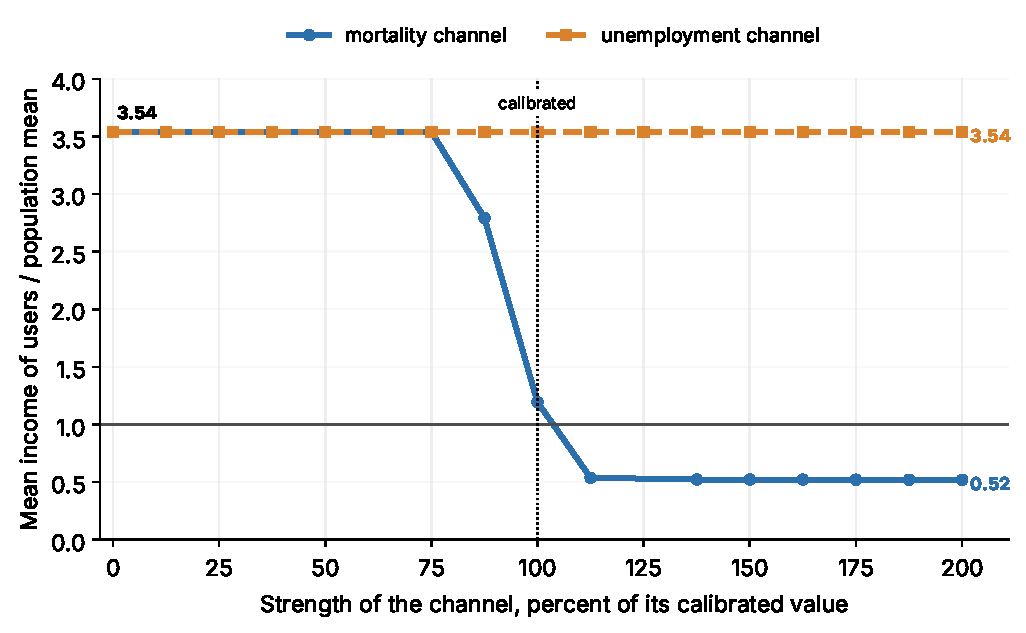
\includegraphics[width=0.83\textwidth]{stylized_who_uses.pdf}
\begin{itemize}\small
\item No consequences: the average user earns \textbf{3.51} times the mean (a luxury good)
\item Mortality alone: \textbf{0.64} at calibrated strength (crosses the mean at 73\pc); unemployment alone: stays at \textbf{3.51}
\item Without saving, unemployment alone also reverses it: \textbf{0.75}
\end{itemize}
\note{Participation is held at 8.90 percent throughout, by recalibrating b, so only who uses changes.}
\end{frame}

\begin{frame}{Why: a penalty rises with income only if it cannot be insured}
\begin{itemize}\setlength\itemsep{0.6em}
\item The utility cost of the drug \alert{falls} with income: a richer household gives up less marginal utility per dollar
\item Losing a job: a richer household saves more to protect itself, so its loss is roughly proportional to its income $\Rightarrow$ the same utility cost for rich and poor
\item Dying: wipes out the whole continuation value of being alive, which \alert{rises} with income $\Rightarrow$ deters the rich, not the poor
\item Life insurance protects descendants, not the household's own life
\item Without saving, job loss also grows with income, which is why it then reverses the gradient as well
\end{itemize}
\note{Two things vary with income: the cost of acquiring the drug and the penalty the drug inflicts.}
\end{frame}

% =============================================================================== quantitative model
\section{The quantitative model}

\begin{frame}{Quantitative model: environment}
Keeps the stylized model's preferences and the two risks of a SUD, and adds:
\begin{itemize}\setlength\itemsep{0.3em}
\item Annual periods, life cycle, income and unemployment risk, unemployment insurance, retirement, progressive taxes
\item Housing: a free shelter or street $h_1$ and three rental sizes $h_2<h_3<h_4$; rationed, means-tested vouchers
\item A drug-use decision every year; recovery; costly, publicly funded treatment $\tau$
\item SMI, likelier with a SUD; it lowers job finding and recovery and raises mortality
\item Homelessness raises mortality, worsens employment and lowers recovery
\item Children who live with their parent for $J_K$ years
\item An endogenous drug price; a budget held at its benchmark net revenue
\end{itemize}
State $(j,a,y,e,d,m,\eta)$, with $d\in\{$never, recovered, current$\}$ and voucher standing $\eta\in\{$none, holder, excluded$\}$
\note{The SUD keeps its history because the parent's valuation of its child depends on whether the disorder was present while the child lived at home.}
\end{frame}

\begin{frame}{Preferences: the child shares the bundle but not the drug}
\[
X_P=\Big[\Big(\tfrac{c}{\xi(j)}\Big)^{1-\gamma}\Big(\tfrac{h}{\xi(j)}\Big)^{\gamma}\Big]^{1-\theta}(b+v)^{\theta},
\qquad
X_c=\Big[\Big(\tfrac{c}{\xi(j)}\Big)^{1-\gamma}\Big(\tfrac{h}{\xi(j)}\Big)^{\gamma}\Big]^{1-\theta}b^{\theta}
\]
\[
u(c,h,v,\tau)=U(X_P)+\omega_c\,(\xi(j)-1)\,U(X_c)+\aleph-\tau\,\bar\tau^{u}
\]
\begin{itemize}\setlength\itemsep{0.35em}
\item Equivalence scale $\xi(j)$: two members while the child is at home, one after
\item $\omega_c<1$: the parent counts only part of its child's welfare
\item No preference parameter varies with the SUD, SMI or housing: the disorder works only through what it costs
\end{itemize}
\note{Varying preferences with the disorder would make reducing addiction and housing people complements mechanically.}
\end{frame}

\begin{frame}{The SUD, recovery and the child's penalty}
\begin{align*}
\Pr(d'=2\mid d\neq2,v)&=\pi_d\,\mathbf{1}\{v>0\}\\
\pi_r(h,m,\tau)&=\min\big\{1,\ \bar\pi_r\,\mu_H^{\mathbf{1}\{h=h_1\}}\,\mu_m^{\mathbf{1}\{m=1\}}\,g^{\mathbf{1}\{\tau=1\}}\big\}
\end{align*}
\vspace{-0.2cm}
Child's productivity at entry:
\[
\begin{aligned}
\log y_{1}^{\text{child}}=\ &\rho\log y^{\text{parent}}+(1-\rho)\mu+\epsilon\\
&+\log(1-\delta_d)\,\mathbf{1}\{\text{parent had a SUD while the child was at home}\}
\end{aligned}
\]
What the parent's disorder costs the child, in its own lifetime value:
\[
D(y,d)=\mathbb{E}\big[V(1,s_{\text{child}})\mid y,0\big]-\mathbb{E}\big[V(1,s_{\text{child}})\mid y,d\big]\ \ge 0
\]
\note{The child inherits a worse productivity draw, not a taste for drugs. D is a difference, so a parent who never had the disorder is charged nothing.}
\end{frame}

\begin{frame}{The household's problem}
\[
\begin{aligned}
V(j,s)=\max_{\{h,\,v,\,\tau,\,a'\}}\ \Big\{\
&U(X_P)+\omega_c(\xi(j)-1)\,U(X_c)+\aleph-\tau\bar\tau^{u}\\
&+\ \beta\,\phi(j,h,d,m)\int V(j{+}1,s')\,\Gamma(\mathrm{d}s'\mid s,h,v,\tau,a')\\
&-\ \beta\,\chi(j)\,\omega_c\,D(y,d)\Big\}
\end{aligned}
\]
\[
\text{s.t.}\quad c+p_v v+a'=y^{n}+a+T_0\mathbf{1}\{j=1\}-p_r h\,\mathbf{1}\{h\neq h_1\}+V\!ch+F
\]
\begin{itemize}
\item $\chi(j)$: the chance the child leaves home after this period, at the parent's death before $J_K$ or at $J_K$
\item The parent is charged $\omega_c D(y,d)$ when its child leaves; the rest of $D$ is an externality
\end{itemize}
\note{Mortality depends on drug use and on housing, so the child enters the drug and housing decisions every year, not only at a terminal date.}
\end{frame}

\begin{frame}{Vouchers and the two policies}
\begin{itemize}\setlength\itemsep{0.4em}
\item Eligible while $\hat y<\kappa_V\,y^{\text{med}}$; an eligible household without a voucher draws one with probability $\pi_V$; a holder keeps it while eligible
\item \textbf{\HF{}}: that is the whole rule
\item \textbf{\TF{}}: holders and new draws are tested; a household fails if it uses, or has a SUD and is not in treatment
\begin{itemize}
\item Treatment is publicly funded; no one may use, even in treatment (Executive Order 14321 and its guidance)
\item A failure is caught with probability $p_{\text{det}}<1$; each test costs $c_{\text{test}}$
\item A caught household loses the voucher and is excluded, returning to the lottery with probability $\psi_x$ a year
\end{itemize}
\item $p_{\text{det}}$, $\psi_x$ and $c_{\text{test}}$ bind only in the experiment
\end{itemize}
\note{A detected holder keeps this period's payment and loses the voucher from the next; a detected applicant never receives it.}
\end{frame}

\begin{frame}{Government, drug market and equilibrium}
\textbf{Drug market}: the price clears a supply curve
\[
p_v=\nu_1 S_v^{1/\varepsilon_s},\qquad S_v=\sum_j\int v(j,s)\,\mathrm{d}\Phi(j,s)
\]
\textbf{Government}: labour and capital income taxes and estates of the dead fund UI, social security, food assistance, vouchers, drug tests and treatment; tax rates are held fixed
\vspace{0.3cm}

\textbf{Equilibrium}: at every date, households optimise, the distribution follows its law of motion,
\begin{itemize}
\item $p_v$ clears the drug market
\item $\pi_V$ holds net government revenue at its benchmark level
\end{itemize}
\vspace{0.2cm}
Either can be switched off: this separates the micro effects a trial sees from the macro effects it cannot
\note{Suppliers are outside the economy. Average income, median income and the fair market rent are held at their benchmark values.}
\end{frame}

% =============================================================================== calibration
\section{Calibration and validation}

\begin{frame}{Calibration strategy}
\begin{itemize}\setlength\itemsep{0.5em}
\item 59 parameters: 38 set externally from data or the literature, 21 calibrated internally
\item 26 carry the story, in six blocks: who uses drugs; costs of homelessness and vouchers; SMI; recovery and treatment; externalities; the drug market
\item The other 33 are standard life-cycle parameters
\item Three parameters bind only in the experiment: detection $p_{\text{det}}$, exclusion $\psi_x$, test cost $c_{\text{test}}$
\item Every target and its dataset, year and universe are documented in the replication package
\end{itemize}
\note{Each parameter is described in the paper by what it controls, its link to the policies, what happens as it rises, and then its target and source.}
\end{frame}

\begin{frame}{Selected parameters and targets}
\centering\footnotesize
\resizebox{\textwidth}{!}{\begin{tabular}{@{}llrrr@{}}
\toprule
Parameter & Moment and source & Data & Model & Value\\
\midrule
$b$, first unit's marginal utility & Any drug use disorder, NSDUH 2024 & 8.90\% & 8.96\% & 0.0054\\
$\pi_d$, chance use leads to a SUD & Share of users with a SUD, NSDUH 2024 & 41.3\% & 42.6\% & 0.0345\\
$\kappa_{\phi d}$, mortality with a SUD & Users' income over average, NSDUH 2024 & 74\% & 62\% & 4.00\\
$\aleph$, value of being alive & VSL, Viscusi and Aldy (2003) & 80 & 81 & 87.6\\
$h_1$, service flow of homelessness & Homelessness, HUD PiT and Burt et al.\ (2001) & 0.40--1.00\% & 0.62\% & 0.0216\\
$\pi_V$, chance of drawing a voucher & Recipients over eligible, HUD 2023 & 26.6\% & 27.5\% & 0.0675\\
$\mu_H$, recovery when homeless & Abstinence, housed/homeless, Milby et al.\ (2005) & 1.47 & 1.45 & 0.696\\
$\bar\tau^{u}$, utility cost of treatment & Treatment take-up, NSDUH 2024 & 24.5\% & 24.9\% & 4.49\\
$\omega_c$, parent's weight on its child & Two-adult over lone-parent use, NSDUH 2024 & 17.5\% & 17.7\% & 0.085\\
$\delta_d$, child's earnings loss & Earnings lost in utero, Nilsson (2017) & 0.24 & n.a. & 0.24\\
$\varepsilon_s$, supply elasticity & Mace et al.\ (2020) & 1.46 & n.a. & 1.46\\
\bottomrule
\end{tabular}}
\source{Table 3 of the paper; Model is the \HF{} benchmark.}
\note{Users' income falls short of its target, 62 against 74 percent; the validation shows where the gap comes from.}
\end{frame}

\begin{frame}{Disciplining the externalities}
\textbf{Parent's weight on its child}, $\omega_c=0.085$
\begin{itemize}
\item NSDUH 2024: an unmarried adult living with another adult and no child is 17.5\pc{} more likely to use than a lone parent with one child, reweighted to the same age, sex, marital status and income
\item The model matches it as the rise in use when the child gets no weight (17.7\pc)
\item At Nishiyama's (2000) 0.69, \TF{} still raises a newborn's welfare, by 3.18\pc
\end{itemize}
\vspace{0.2cm}
\textbf{Child's earnings penalty}, $\delta_d=0.24$
\begin{itemize}
\item The earnings loss at age 32 that Nilsson (2017) measures for children of mothers under 21 exposed in utero to a Swedish alcohol experiment
\item The earnings externality is only 18\pc{} of the gain; with no penalty \TF{} still gains
\end{itemize}
\note{With a weight of 0.69, less of the gain is an externality, 23 percent against 76, because the parent counts most of what its choices cost the child.}
\end{frame}

\begin{frame}{Disciplining the screen}
\textbf{Detection rate} $p_{\text{det}}$: set so the screen deters as much as the closest evidence
\begin{itemize}\setlength\itemsep{0.4em}
\item US military random drug testing with dismissal: those who stayed were 61\pc{} less likely to use marijuana (Mehay and Pacula, 1999)
\item In the model, with $p_{\text{det}}=20\pc$, 62\pc{} of the users facing the screen stop when it is introduced, and none starts
\item Compared as proportional responses, since the military measure is broader
\item At half the rate, 41\pc{} stop, inside the 11 to 45\pc{} range once leavers are counted; a newborn still gains 1.65\pc
\item A test costs \$35 (Texas Legislative Budget Board, 2013), the upper end of the estimates; exclusion lasts three years on average
\end{itemize}
\note{The counterpart applies Treatment First to the Housing First distribution, drug price and pi_V, and follows each user who faces the screen. A positive screen is confirmed in a laboratory, so a non-user is never flagged.}
\end{frame}

\begin{frame}{Validation: untargeted moments}
\centering\footnotesize
\resizebox{\textwidth}{!}{\begin{tabular}{@{}lrrl@{}}
\toprule
Moment & Data & Model & Source\\
\midrule
Abstinence, contingent over unconditional housing, ratio & 1.26 & 1.40 & Milby et al.\ (2005)\\
Three-year mortality, households with SMI put on the street, pp & 4.6 & 3.6 & Costantini (2025)\\
Child of a SUD parent acquires a SUD, odds ratio & 1.44, 2.51 & 1.46 & Mellentin et al.; Yoon et al.\\
Children living with a parent with a SUD, \% & 4.6 & 5.8 & NSDUH 2024\\
Unemployment given a SUD, \% & 16.2 & 14.5 & NSDUH 2024\\
Drug use with SMI over without, ratio & 2.44 & 2.64 & NSDUH 2024\\
Participation price elasticity & $-0.3$ to $-0.9$ & $-1.32$ & Saffer and Chaloupka (1999)\\
Intensive price elasticity, users & $-0.3$ to $-0.8$ & $-0.63$ & Grossman and Chaloupka (1998)\\
Homeless adult had a homeless parent, odds ratio & 1.8 to 2.4 & 6.23 & Bassuk et al.\ (1997)\\
Employed share of the homeless, \% & 46 & 21.4 & Meyer et al.\ (2024)\\
\bottomrule
\end{tabular}}
\source{Table 4 of the paper.}
\note{A larger price response can only work against Treatment First, since it lowers the drug price and draws households back into use. The homelessness odds ratio and the employment of the homeless are misses.}
\end{frame}

\begin{frame}{Validation: drug use by income}
\begin{columns}[T]
\column{0.6\textwidth}
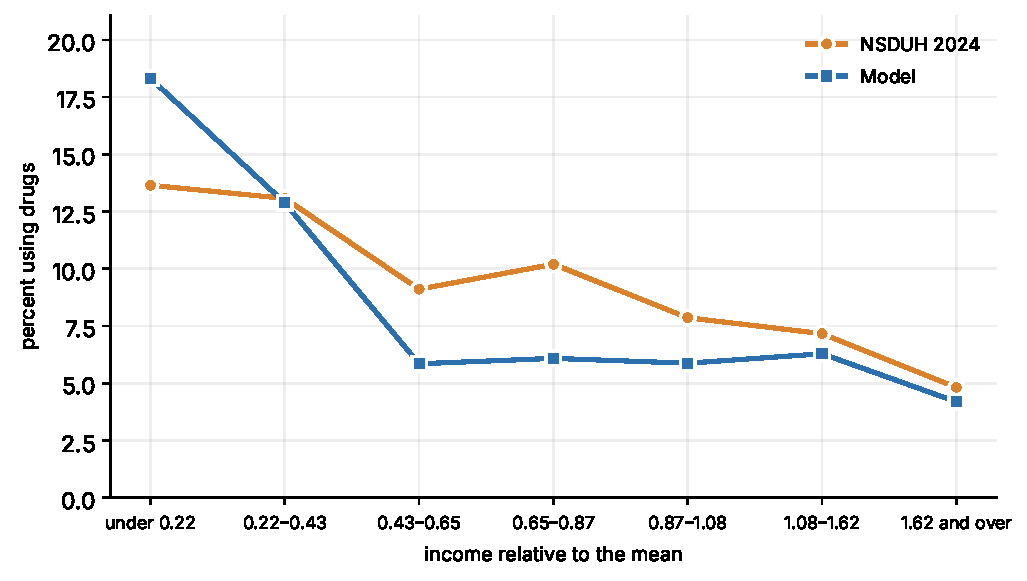
\includegraphics[width=\linewidth]{use_by_income.pdf}
\column{0.37\textwidth}\small
\begin{itemize}\setlength\itemsep{0.4em}
\item Only users' average income is targeted
\item Bottom band: 18.3\pc{} use in the model, 13.7\pc{} in NSDUH 2024
\item Top band: 4.2\pc{} against 4.8\pc
\item Middle: flatter and lower, 5.9 to 6.3\pc{} against 7.2 to 10.2\pc
\item Vouchers are means-tested, so the lower users sit, the more of them, and of their children, the screen reaches
\end{itemize}
\end{columns}
\source{NSDUH 2024: adults 26+ with a SUD of any severity, by personal income band relative to the mean of band midpoints.}
\note{Both differences lower users' average income in the model, which is why it falls slightly short of its 74 percent target.}
\end{frame}

% =============================================================================== results
\section{Long-run results}

\begin{frame}{Experiments}
Replace \HF{} with \TF{}; keep the programme rationed and taxes fixed
\begin{enumerate}\setlength\itemsep{0.5em}
\item \textbf{Moral hazard alone}: children removed from welfare and from the parent's preferences, their productivity independent of the parent
\item \textbf{With the children}: the calibrated model, in three steps: the screen alone; then $\pi_V$ clears the budget; then the drug price clears too (the main experiment)
\item \textbf{Transition}: every cohort alive at the reform, with $p_v$ and $\pi_V$ clearing every year
\end{enumerate}
\vspace{0.3cm}
Welfare: consumption-equivalent variation (CEV) of a newborn, childhood included
\[
W_t=\underbrace{\textstyle\sum_{j=1}^{J_K}\beta^{j-1}(\xi(j)-1)\,\mathbb{E}\,U(X_c)}_{\text{childhood}}+\underbrace{\beta^{J_K}\,\mathbb{E}\,V(1,s)}_{\text{adult life}}
\]
\note{Moral hazard here is the textbook definition: Housing First insures a household against losing its home when use leads to a SUD, so part of the cost of using falls on the budget.}
\end{frame}

\begin{frame}{Experiment 1: moral hazard alone does not justify conditionality}
\begin{columns}[T]
\column{0.5\textwidth}
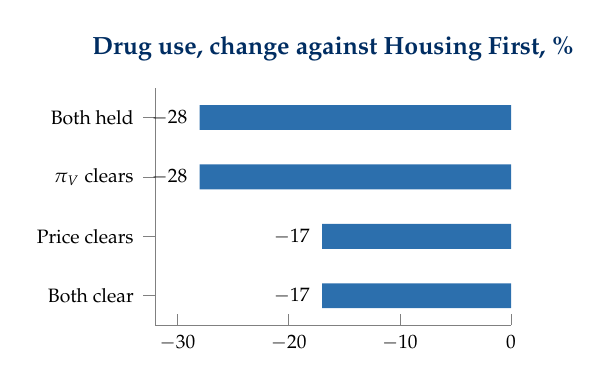
\begin{tikzpicture}
\begin{axis}[acad, xbar, width=6.1cm, height=4.6cm, bar width=9pt, xmin=-32, xmax=0,
  ytick={1,2,3,4}, yticklabels={Both clear, Price clears, $\pi_V$ clears, Both held}, ymin=0.5, ymax=4.5,
  title={Drug use, change against \HF, \%}, nodes near coords, nodes near coords align={horizontal},
  every node near coord/.append style={anchor=east, xshift=-1pt}]
\addplot[fill=hfblue, draw=none] coordinates {(-28,4) (-28,3) (-17,2) (-17,1)};
\end{axis}
\end{tikzpicture}
\column{0.5\textwidth}
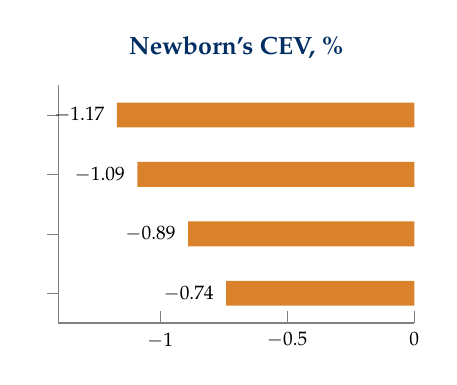
\begin{tikzpicture}
\begin{axis}[acad, xbar, width=6.1cm, height=4.6cm, bar width=9pt, xmin=-1.4, xmax=0,
  ytick={1,2,3,4}, yticklabels={}, ymin=0.5, ymax=4.5,
  title={Newborn's CEV, \%}, nodes near coords, nodes near coords align={horizontal},
  every node near coord/.append style={anchor=east, xshift=-1pt, /pgf/number format/fixed, /pgf/number format/precision=2, /pgf/number format/fixed zerofill}]
\addplot[fill=tforange, draw=none] coordinates {(-1.17,4) (-1.09,3) (-0.89,2) (-0.74,1)};
\end{axis}
\end{tikzpicture}
\end{columns}
\small
\begin{itemize}
\item Rows: the drug price and $\pi_V$ held at their \HF{} levels or allowed to clear
\item Use falls by up to 28\pc, yet a newborn loses in every case: the screen removes an option from households that weigh the risks correctly, and the budget gives little back (with $\pi_V$ clearing, 58\pc{} gain, by 0.05\pc{} on average; 96\pc{} of those with a SUD lose)
\end{itemize}
\note{With the price clearing, the newborn loses less, 0.74 percent, but that is the general-equilibrium effect of a cheaper drug, not a correction of moral hazard.}
\end{frame}

\begin{frame}{Experiment 2: count the children and every step gains}
\centering
\resizebox{\textwidth}{!}{\begin{tabular}{@{}lccc@{}}
\toprule
 & Screen alone & + $\pi_V$ clears & + price clears (main)\\
\midrule
Newborn's CEV, \% of lifetime consumption & 2.82 & 6.45 & \textbf{2.57}\\
Parent's own gain, \% & $-$1.19 & 2.42 & 0.69\\
Drug use, change against \HF, \% & $-$43 & $-$42 & $-$21\\
Homelessness, change against \HF, \% & $-$8 & $-$20 & $-$11\\
$\pi_V$, \% (benchmark 6.75) & 6.75 & 9.24 & 7.80\\
\bottomrule
\end{tabular}}
\vspace{0.4cm}
\raggedright
\begin{itemize}
\item Screen alone: parents lose about what they lose without children, but the child gains more than its parent loses
\item Recycling the savings into vouchers makes parents gain too
\item The cheaper drug (price $-$5\pc) draws some users back, which takes part of the gain away
\end{itemize}
\note{With the price clearing and pi_V held, the newborn gains 0.98 percent: the freed revenue goes unspent. The main experiment is the last column, because after a real reform both the price and the budget would adjust.}
\end{frame}

\begin{frame}{Main experiment: every outcome falls, childhood homelessness included}
\centering
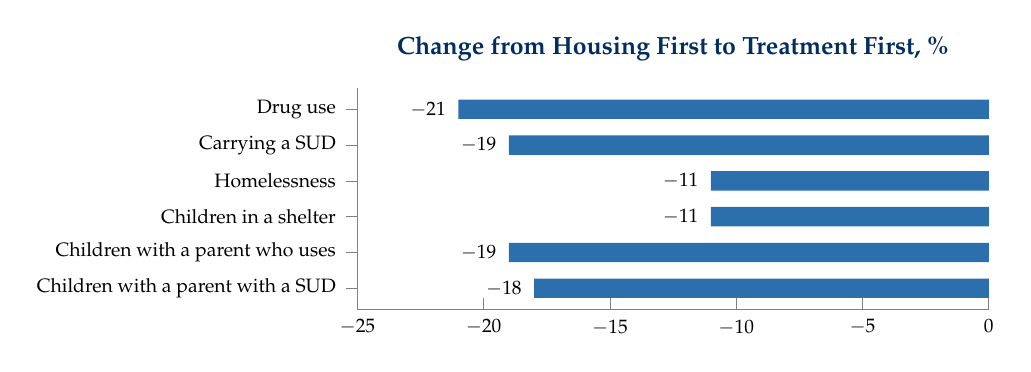
\begin{tikzpicture}
\begin{axis}[acad, xbar, width=9.6cm, height=4.4cm, bar width=7pt, xmin=-25, xmax=0, ymin=0.4, ymax=6.6,
  ytick={1,...,6}, yticklabels={Children with a parent with a SUD, Children with a parent who uses, Children in a shelter, Homelessness, Carrying a SUD, Drug use},
  title={Change from \HF{} to \TF, \%},
  nodes near coords, nodes near coords align={horizontal}, every node near coord/.append style={anchor=east, xshift=-1pt}]
\addplot[fill=hfblue, draw=none] coordinates {(-21,6) (-19,5) (-11,4) (-11,3) (-19,2) (-18,1)};
\end{axis}
\end{tikzpicture}
\raggedright\small
\begin{itemize}
\item Drug use 8.92 $\to$ 7.07\pc; homelessness 0.62 $\to$ 0.55\pc; children in a shelter 1.03 $\to$ 0.92\pc
\item $\pi_V$ +16\pc, to 7.80\pc; drug price $-$5\pc; treatment among those with a SUD 24.6 $\to$ 29.0\pc
\end{itemize}
\note{Tax revenue rises mainly because more children start adult life with higher productivity. A household with a SUD keeps its voucher by entering treatment and stopping; when it cannot respond at all, the results still hold.}
\end{frame}

\begin{frame}{Why homelessness falls}
\begin{enumerate}\setlength\itemsep{0.6em}
\item Households that stop using spend less on drugs, so more of them can house themselves
\item Less SUD means less unemployment, and so less homelessness
\item The vouchers revoked from households with a SUD go, through a higher $\pi_V$, to other low-income households
\end{enumerate}
\vspace{0.4cm}
Among households aged 26 to 50, the years a child lives at home, homelessness also falls by 11\pc{}\\[0.3em]
$\Rightarrow$ no trade-off between the externalities: by cutting use, the screen keeps more children out of a shelter than it sends to one
\note{This is the externality critics of Treatment First worry about, and it goes the other way.}
\end{frame}

\begin{frame}{Where the gain comes from}
\[
\Delta W=\underbrace{(1-\omega_c)\Delta C}_{\text{childhood externality}}+\underbrace{(1-\omega_c)\Delta E}_{\text{earnings externality}}+\underbrace{\beta^{J_K}\Delta P}_{\text{own adult life}}+\underbrace{\omega_c(\Delta C+\Delta E)}_{\text{counted by the parent}}
\]
\centering\small
\begin{tabular}{@{}lccc@{}}
\toprule
 & Both held & $\pi_V$ clears & Both clear\\
\midrule
Newborn's gain $\Delta W$, \% of lifetime consumption & 2.82 & 6.45 & \textbf{2.57}\\
\quad Childhood its parent does not count & 2.20 & 3.47 & 1.50\\
\quad Productivity at entry its parent does not count & 1.06 & 1.00 & 0.46\\
\quad Own adult life under the policy & $-$0.75 & 1.54 & 0.43\\
\quad What its parent does count & 0.31 & 0.44 & 0.19\\
\midrule
Externality, \% of the gain & 116 & 69 & \textbf{76}\\
Parent's own gain, \% of its lifetime consumption & $-$1.19 & 2.42 & 0.69\\
\bottomrule
\end{tabular}
\source{Table 6 of the paper. The childhood part is the largest: it accrues every year at home; the penalty reaches the child once.}
\note{With prices held, the newborn's own adult life is a loss, so the externality is more than all of the gain. In general equilibrium both the child and the parent gain.}
\end{frame}

\begin{frame}{Who gains, and why trials point the other way}
\begin{itemize}\setlength\itemsep{0.5em}
\item 99.9\pc{} of households entering adult life are better off: the screen costs them nothing unless they choose to use
\item 74\pc{} of all households are better off and 3\pc{} worse off; 24\pc{} of those with a SUD are better off
\item What a trial sees: those with a SUD when the reform lands lose; 74\pc{} are worse off with the price and $\pi_V$ held, as in a trial too small to move either, 67\pc{} once both clear
\item What it cannot see: the households the condition deters from ever starting, the vouchers its savings buy for others, and the children's adult lives
\end{itemize}
\vspace{0.2cm}
$\Rightarrow$ the model agrees with the micro evidence on the households it follows; the macro effects overturn the verdict
\note{The trials follow adults who are already homeless, most with SMI and many with a SUD.}
\end{frame}

% =============================================================================== transition
\section{The transition}

\begin{frame}{The transition from \HF{} to \TF}
\begin{columns}[T]
\column{0.5\textwidth}
\centering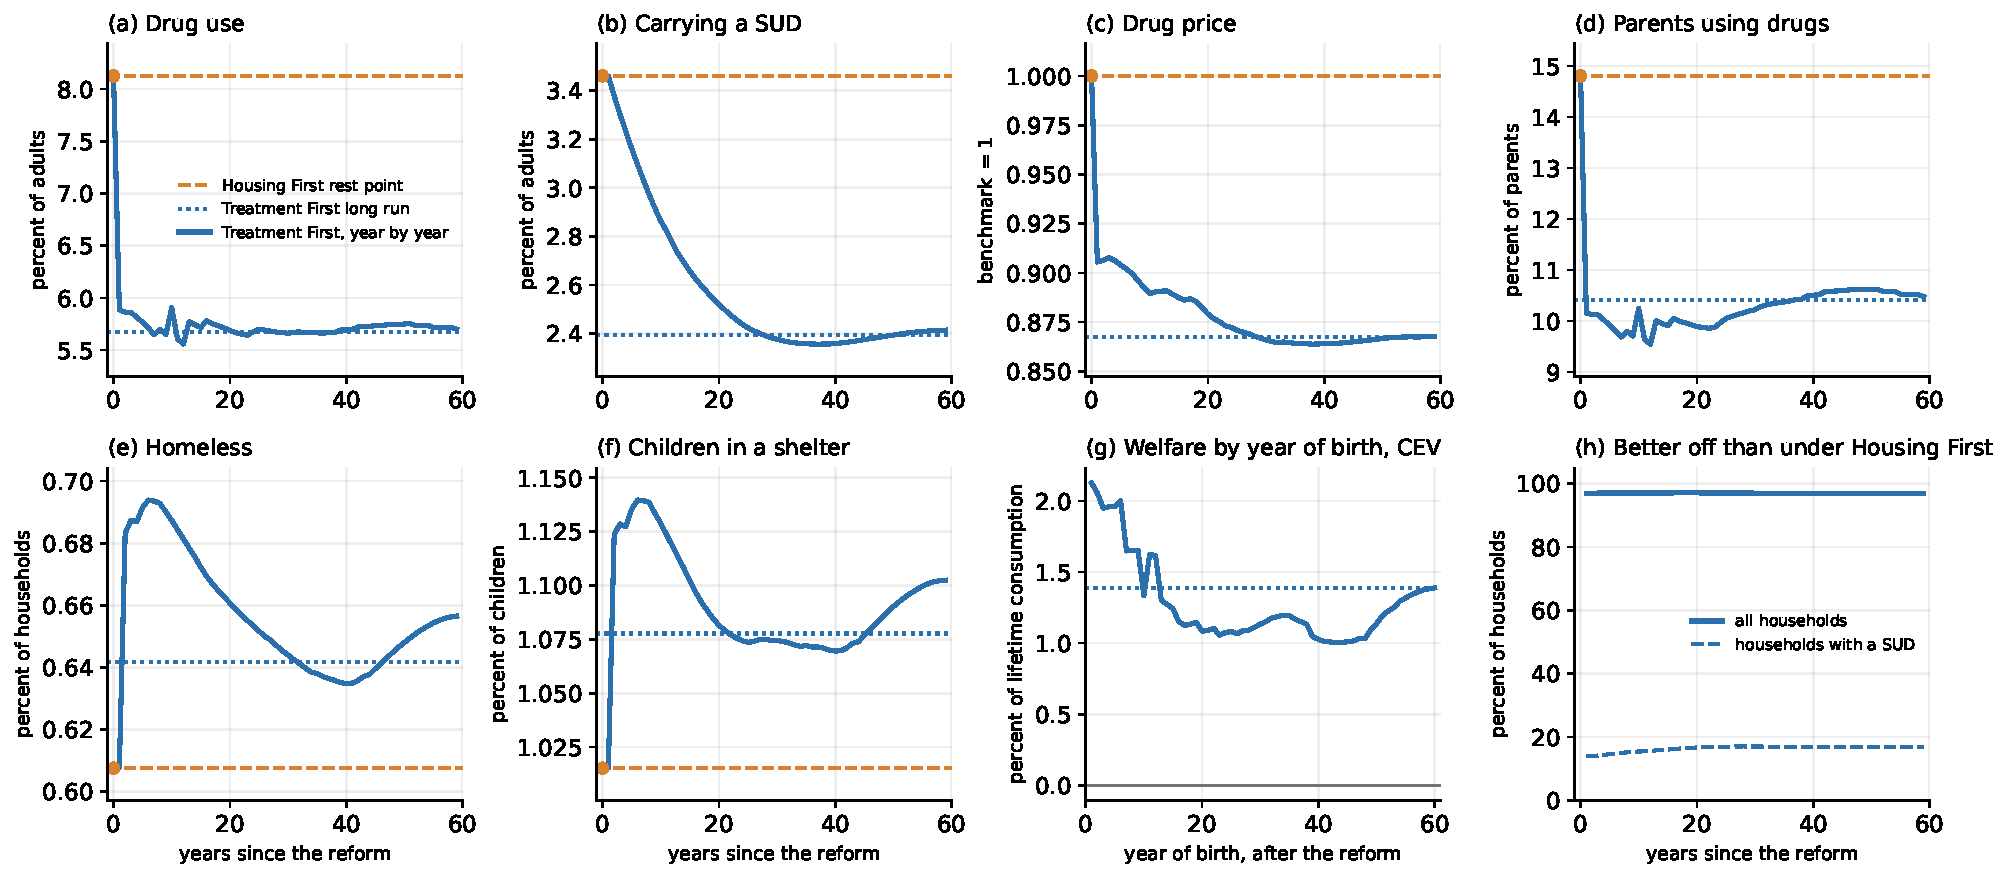
\includegraphics[height=0.8\textheight]{full_transition.pdf}
\column{0.47\textwidth}\small
\begin{itemize}\setlength\itemsep{0.4em}
\item Unexpected, permanent reform in year 1; all cohorts alive; $p_v$ and $\pi_V$ clear every year
\item 81\pc{} of the fall in drug use happens in year 1; SUD falls slowly (half by year 11)
\item Homelessness 0.62 $\to$ 0.60 (year 10) $\to$ 0.55\pc; children in a shelter 1.03 $\to$ 1.00 $\to$ 0.92\pc: \alert{neither ever rises}
\item Children born at the reform gain 1.45\pc; 11\pc{} of adults alive at the reform lose
\end{itemize}
\end{columns}
\note{The drug price stays above its long-run level for 33 years because those who still have a SUD keep demand up. Children born at the reform gain less because the SUD falls only as fast as recovery allows and pi_V is lower in the first decade.}
\end{frame}

\begin{frame}{Why homelessness does not rise in the first years}
\begin{enumerate}\setlength\itemsep{0.6em}
\item \textbf{Few lose a voucher}: a household with a SUD keeps it by entering treatment and not using, and the screen catches a user 20\pc{} of the time; at most 0.13\pc{} of households are excluded in any year
\item \textbf{Drug use falls at once}: households spend less on drugs and have more left for housing, and fewer acquire a SUD and the unemployment it brings
\item \textbf{Vouchers are recycled}: after the first three years, when it dips to 6.55\pc, $\pi_V$ stays above its \HF{} level of 6.75\pc
\end{enumerate}
\vspace{0.3cm}
The first reason depends on design: it needs treatment and sobriety to be a real option for those who already have a SUD
\note{The next slide drops that assumption.}
\end{frame}

\begin{frame}{Alternative transitions: those with a SUD cannot stop using}
\begin{columns}[T]
\column{0.56\textwidth}
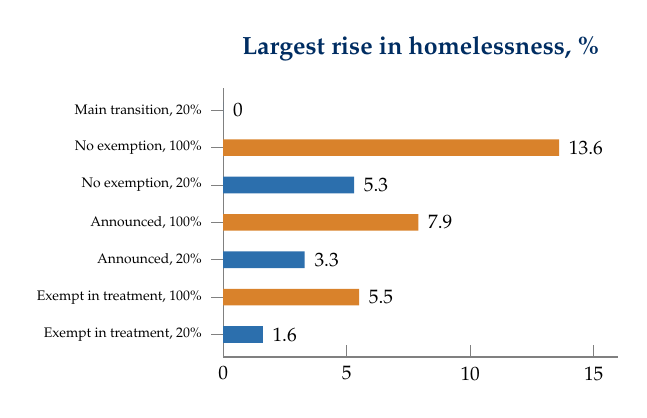
\begin{tikzpicture}
\begin{axis}[acad, xbar, width=6.6cm, height=5.0cm, bar width=6pt, bar shift=0pt, xmin=0, xmax=16,
  ytick={1,...,7}, ymin=0.4, ymax=7.6,
  yticklabels={Exempt in treatment{,} 20\%, Exempt in treatment{,} 100\%, Announced{,} 20\%, Announced{,} 100\%, No exemption{,} 20\%, No exemption{,} 100\%, Main transition{,} 20\%},
  y tick label style={font=\tiny}, title={Largest rise in homelessness, \%},
  nodes near coords, nodes near coords align={horizontal}]
\addplot[fill=tforange, draw=none] coordinates {(13.6,6) (7.9,4) (5.5,2)};
\addplot[fill=hfblue, draw=none] coordinates {(0,7) (5.3,5) (3.3,3) (1.6,1)};
\end{axis}
\end{tikzpicture}
\column{0.42\textwidth}
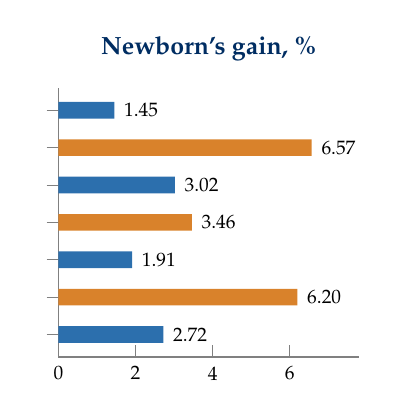
\begin{tikzpicture}
\begin{axis}[acad, xbar, width=5.4cm, height=5.0cm, bar width=6pt, bar shift=0pt, xmin=0, xmax=7.8,
  ytick={1,...,7}, yticklabels={}, ymin=0.4, ymax=7.6, title={Newborn's gain, \%},
  nodes near coords, nodes near coords align={horizontal},
  every node near coord/.append style={/pgf/number format/fixed, /pgf/number format/precision=2, /pgf/number format/fixed zerofill}]
\addplot[fill=tforange, draw=none] coordinates {(6.57,6) (3.46,4) (6.20,2)};
\addplot[fill=hfblue, draw=none] coordinates {(1.45,7) (3.02,5) (1.91,3) (2.72,1)};
\end{axis}
\end{tikzpicture}
\end{columns}
\small
\begin{itemize}
\item Orange: the screen catches every user; blue: one in five. A five-period exemption in treatment holds the rise to 1.6\pc, and newborns still gain more than in the main transition
\end{itemize}
\note{Catching every user with no exemption keeps homelessness above Housing First for fifteen years. Announcing the screen cuts drug use by 15 percent before it starts, but the rise comes when it does.}
\end{frame}

% =============================================================================== conclusion
\section{Robustness and conclusion}

\begin{frame}{Robustness}
\centering\small
\begin{tabular}{@{}>{\raggedright\arraybackslash}p{6.2cm}>{\raggedright\arraybackslash}p{7.2cm}@{}}
\toprule
Change & Result\\
\midrule
Detection at half the rate, 10\% & Newborn +1.65\%; use $-$14\%, homelessness $-$6\%\\
Those with a SUD cannot respond at all & Use $-$29\%, homelessness $-$11\%; newborn gains at least as much\\
Parent's weight on the child at 0.69 (Nishiyama, 2000) & Newborn +3.18\%, 23\% of it an externality\\
No earnings penalty for the child & \TF{} still raises welfare; the earnings externality is 18\% of the gain\\
A disamenity of homelessness (Loubi\`ere et al., 2020) & No long-run gain moves by more than 0.14 pp\\
Log utility in the stylized model & All qualitative results hold\\
\bottomrule
\end{tabular}
\note{Each row changes one thing and re-solves the model.}
\end{frame}

\begin{frame}{Conclusion}
\textbf{Should housing assistance require sobriety?}
\begin{itemize}
\item \alert{Yes}, if the externalities on children are counted; \alert{no}, if the case rests on moral hazard
\end{itemize}
\vspace{0.2cm}
\textbf{Three lessons}
\begin{enumerate}\setlength\itemsep{0.4em}
\item Both sides of the debate leave out what matters most: the children of the households a sobriety requirement deters, in what they consume, whether they become homeless and what they earn as adults
\item The model agrees with the trials on the households they follow, who lose from the condition; the macro effects the trials cannot capture overturn the conclusion
\item Homelessness does not fall along the way unless treatment and sobriety are a real option for those who already have a SUD; a temporary exemption in treatment keeps childhood homelessness from ever rising
\end{enumerate}
\note{Moral hazard is the argument that dominates the policy debate, and on its own it does not justify the screen. What does is the cost of a parent's drug use to a child that the parent counts only in part.}
\end{frame}

{\setbeamertemplate{footline}{}
\begin{frame}
\centering\vfill
{\Large\bfseries\color{dblue}Thank you}\par\vspace{0.4cm}
Shahar Rotberg\par
{\small Canada Mortgage and Housing Corporation}\par
\vfill
\end{frame}}

% =============================================================================== backup
\appendix
\section*{Backup}

\begin{frame}{Backup: long-run results in full (Table 5)}
\centering
\resizebox{0.86\textwidth}{!}{% Written by code/paper/export_longrun.py from results/counterfactuals_cf_fix2;
% edit the script, not this file. Caption and note are in the paper.
\begin{tabular}{@{}L{170pt}rrrr@{}}
\toprule
 & Housing & Treatment & \textcolor{red}{Optimal} & \textcolor{red}{Optimal} \\
 & First & First & \textcolor{red}{drug use} & \textcolor{red}{homelessness} \\
\midrule
\multicolumn{5}{@{}l}{\emph{Adults}} \\
Drug price, benchmark $=1$ & 1.00 & 0.87 & 0.86 & \textcolor{red}{1.00} \\
Voucher probability $\pi_V$ & 6.75 & 8.14 & 6.75 & \textcolor{red}{6.75} \\
Drug use & 8.12 & 5.67 & 5.22 & \textcolor{red}{7.96} \\
Carrying a SUD & 3.46 & 2.39 & 2.21 & \textcolor{red}{3.39} \\
Homelessness & 0.61 & 0.64 & 0.53 & \textcolor{red}{0.59} \\
SUD share of the homeless & 19.2 & 21.5 & 11.2 & \textcolor{red}{18.8} \\
In treatment, of those with a SUD & 25.0 & 29.3 & 25.0 & \textcolor{red}{25.1} \\
\addlinespace
\multicolumn{5}{@{}l}{\emph{\textcolor{red}{Children}}} \\
Living with a parent who uses drugs & 14.80 & 10.40 & 9.52 & \textcolor{red}{14.51} \\
Living with a parent who carries a SUD & 5.28 & 3.69 & 3.41 & \textcolor{red}{5.18} \\
In a shelter & 1.02 & 1.08 & 0.85 & \textcolor{red}{0.99} \\
\addlinespace
\multicolumn{5}{@{}l}{\emph{Welfare}} \\
CEV of a newborn, percent of lifetime consumption & -- & 1.39 & -- & \textcolor{red}{--} \\
Share of the newborn's gain that comes in childhood & -- & 50 & -- & \textcolor{red}{--} \\
\bottomrule
\end{tabular}
}
\source{Percent unless stated. Columns 2--5: without externalities, against column 1; columns 7--10: with externalities, against the benchmark in column 6. Detection rate 20\%.}
\end{frame}

\begin{frame}{Backup: alternative transitions in full (Table 7)}
\centering\small
\resizebox{\textwidth}{!}{\begin{tabular}{@{}lcccccc@{}}
\toprule
 & & \multicolumn{2}{c}{Homelessness} & \multicolumn{2}{c}{Children in a shelter} & Newborn's\\
\cmidrule(lr){3-4}\cmidrule(lr){5-6}
 & $p_{\mathrm{det}}$ & Largest rise & Periods above & Largest rise & Periods above & gain\\
\midrule
Main transition & 20 & none & none & none & none & 1.45\\
\addlinespace
No exemption & 100 & 13.6 (2) & 1--15 & 10.8 (2) & 2--11 & 6.57\\
 & 20 & 5.3 (6) & 2--17 & 3.1 (5) & 2--11 & 3.02\\
\addlinespace
Announced five periods ahead & 100 & 7.9 (10) & 7--17 & 4.4 (9) & 7--13 & 3.46\\
 & 20 & 3.3 (12) & 7--19 & 0.9 (10) & 8--13 & 1.91\\
\addlinespace
Treatment exempt, first five periods & 100 & 5.5 (7) & 7--14 & 2.0 (7) & 7--10 & 6.20\\
 & 20 & 1.6 (11) & 8--16 & none & none & 2.72\\
\bottomrule
\end{tabular}}
\source{Largest rise above \HF, percent, with the period it occurs in brackets. The drug price and $\pi_V$ clear every period.}
\end{frame}

\end{document}
